\documentclass[crop,tikz,12pt]{standalone}

\usepackage{bbold}

\usetikzlibrary{arrows.meta}
\usetikzlibrary{shapes.geometric}
\usetikzlibrary{calc}

\definecolor{iconcolor}{RGB}{62,108,169}
\colorlet{mygrey}{white!35!black}

\def\tri{0.25}
\def\ind{0.06}
\def\ichw{0.50}
\def\ichh{0.65}

\tikzset{tsv/.pic={code={
    \fill [fill=iconcolor]       (-\ichw, -\ichh)
        [rounded corners=1pt] -- ( \ichw, -\ichh)
        [sharp corners] --       ( \ichw, \ichh-\tri)
        [sharp corners] --       ( \ichw- \tri,\ichh)
        [rounded corners=1pt] -- (-\ichw, \ichh)
        [rounded corners=1pt] -- cycle;
    \fill [black!5!white]        (-\ichw+\ind,       -\ichh+\ind)
        [rounded corners=1pt] -- ( \ichw-\ind,       -\ichh+\ind)
        [sharp corners] --       ( \ichw-\ind,       \ichh-\tri-\ind/2)
        [sharp corners] --       ( \ichw-\tri-\ind/2,\ichh-\tri-\ind/2)
        [sharp corners] --       ( \ichw-\tri-\ind/2,\ichh-\ind)
        [rounded corners=1pt] -- (-\ichw+\ind,       \ichh-\ind)
        [rounded corners=1pt] -- cycle;
    \node [
        draw=black!5!white,
        line width=1pt,
        fill=iconcolor,
        rounded corners=0.5pt,
        scale=0.5,
        text=white]
    at (-\ichw*1/3, -\ichh*1/3) {\hskip 2pt TSV\hskip 2pt\hskip 0pt};
}}}

\tikzset{xref/.pic={code={
    \fill [fill=iconcolor]       (-\ichw, -\ichh)
        [rounded corners=1pt] -- ( \ichw, -\ichh)
        [rounded corners=1pt] -- ( \ichw,  \ichh)
        [rounded corners=1pt] -- (-\ichw,  \ichh)
        [rounded corners=1pt] -- cycle;
    \fill [black!5!white]        (-\ichw+\ind,       -\ichh+\ind)
        [rounded corners=1pt] -- ( \ichw-\ind,       -\ichh+\ind)
        [rounded corners=1pt] -- ( \ichw-\ind,        \ichh-\ind)
        [rounded corners=1pt] -- (-\ichw+\ind,       \ichh-\ind)
        [rounded corners=1pt] -- cycle;
    \node [text=iconcolor,font=\rmfamily\bfseries\LARGE]
    at (-0.05, -0.2) {^^ ^^ };
}}}

\begin{document}

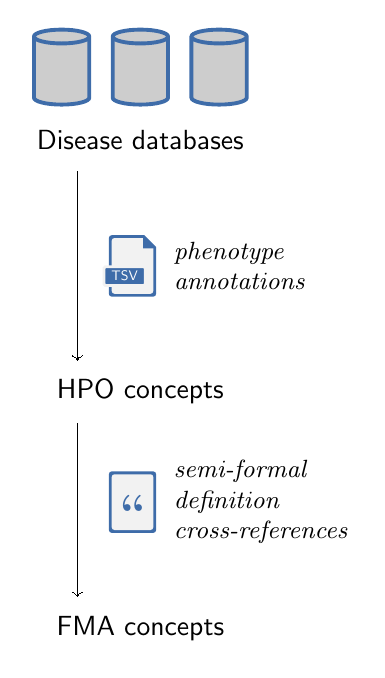
\begin{tikzpicture}[
    every node/.style={font=\sffamily},
    d/.style={fill=mygrey!30!white,line width=1pt,draw=mygrey},
    c/.style={draw=black,line width=0},
    l/.style={
        font=\itshape\small,
        align=left, anchor=west
    },
    a/.style={
        font={}
    },
    database/.style={
        scale=3,
        draw=iconcolor,
        line width=1.4pt,
        cylinder,
        cylinder uses custom fill,
        cylinder body fill=mygrey!30,
        cylinder end fill=mygrey!30,
        shape border rotate=90,
        aspect=0.25,
        draw
    }
]

\node [database] at (-1, 1) {};
\node [database] at ( 0, 1) {};
\node [database] at ( 1, 1) {};

\node (dbs) at (0, 0.2) {Disease databases};
\node (hpo) at (0, -3) {\textbb{HPO} concepts};
\node (fma) at (0, -6) {\textbb{FMA} concepts};

\path [c] (-0.8, -0.2) -- (-0.8, -2.6) [->];
\path (-0.1, -1.4) pic [scale=0.6] {tsv};
\node [l] (ann) at (0.3, -1.4) {phenotype\\annotations};

\path [c] (-0.8, -3.4) -- (-0.8, -5.6) [->];
\path (-0.1, -4.4) pic [scale=0.6] {xref};
% \node [a,rotate=90] at (-0.1, -4.4) {\x};
\node [l] (ann) at (0.3, -4.4) {semi-formal\\definition\\cross-references};

\end{tikzpicture}

\end{document}
